\section{eo\-Real$<$ Fit\-T $>$ Class Template Reference}
\label{classeo_real}\index{eoReal@{eoReal}}
eo\-Real: implementation of simple real-valued chromosome.  


{\tt \#include $<$eo\-Real.h$>$}

Inheritance diagram for eo\-Real$<$ Fit\-T $>$::\begin{figure}[H]
\begin{center}
\leavevmode
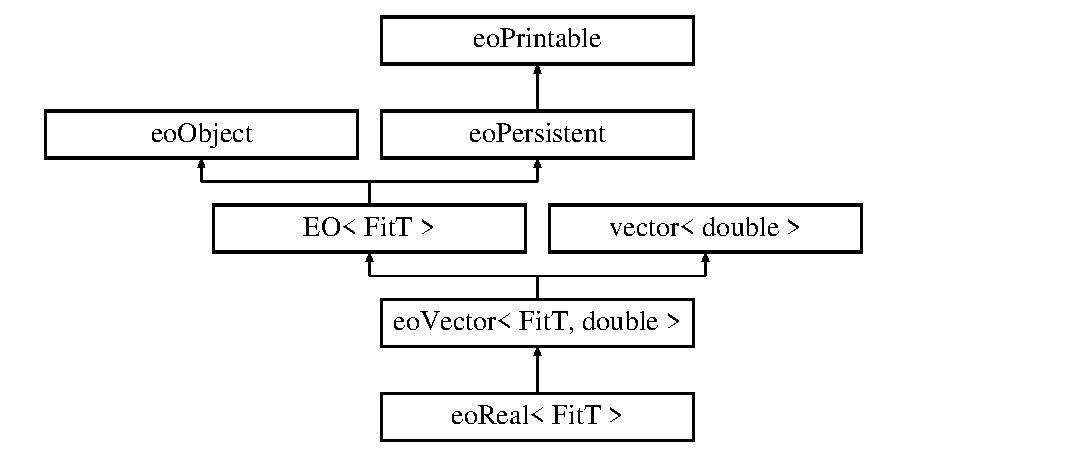
\includegraphics[height=5cm]{classeo_real}
\end{center}
\end{figure}
\subsection*{Public Member Functions}
\begin{CompactItemize}
\item 
{\bf eo\-Real} (unsigned size=0, double value=0.0)
\begin{CompactList}\small\item\em (Default) Constructor. \item\end{CompactList}\item 
virtual std::string {\bf class\-Name} () const \label{classeo_real_a1}

\begin{CompactList}\small\item\em My class name. \item\end{CompactList}\end{CompactItemize}


\subsection{Detailed Description}
\subsubsection*{template$<$class Fit\-T$>$ class eo\-Real$<$ Fit\-T $>$}

eo\-Real: implementation of simple real-valued chromosome. 

based on {\bf eo\-Vector}{\rm (p.\,\pageref{classeo_vector})} class 



Definition at line 37 of file eo\-Real.h.

\subsection{Constructor \& Destructor Documentation}
\index{eoReal@{eo\-Real}!eoReal@{eoReal}}
\index{eoReal@{eoReal}!eoReal@{eo\-Real}}
\subsubsection{\setlength{\rightskip}{0pt plus 5cm}template$<$class Fit\-T$>$ {\bf eo\-Real}$<$ {\bf Fit\-T} $>$::{\bf eo\-Real} (unsigned {\em size} = {\tt 0}, double {\em value} = {\tt 0.0})\hspace{0.3cm}{\tt  [inline]}}\label{classeo_real_a0}


(Default) Constructor. 

\begin{Desc}
\item[Parameters:]
\begin{description}
\item[{\em size}]Size of the std::vector \end{description}
\end{Desc}


Definition at line 45 of file eo\-Real.h.

The documentation for this class was generated from the following file:\begin{CompactItemize}
\item 
eo\-Real.h\end{CompactItemize}
